\documentclass{beamer}
\usetheme{CVUTFIT}
\usepackage{csquotes}
\usepackage{bibentry}
\usepackage{tabularray}
\usepackage[style=iso-numeric]{biblatex}
\addbibresource{bib-database.bib}
\setbeamertemplate{bibliography item}{\insertbiblabel}

\title[Emulátor konzole NES]{Emulátor konzole Nintendo~Entertainment~System}
\subtitle{Bakalářská práce}
\author[Ondřej Golasowski]{Ondřej Golasowski\texorpdfstring{\\}{}Vedoucí práce: Ing.~Stanislav Jeřábek}
\institute[FIT ČVUT]{Katedra číslicového návrhu, FIT ČVUT}
\date{22.~června~2023}


\begin{document}
	
\begingroup
\setbeamertemplate{footline}{}
\begin{frame}[noframenumbering]
	\titlepage
\end{frame}
\endgroup

\section{Úvod}
\begin{frame}
	\frametitle{Představení problematiky}
	\begin{definice}[Emulátor]
		Emulátor je software, který umožňuje běh počítačových programů na jiné platformě, než pro kterou byly původně vytvořeny~\normalfont{\footfullcite{Nash1989:sw-emulator}}.
	\end{definice}
	Rozdíly oproti simulaci:
	\begin{itemize}
		\item Implementuje se pouze model hardwaru
		\item Spouští se původní (neupravený) software
	\end{itemize}
\end{frame}

\begin{frame}
	\frametitle{Motivace a~cíle}
	Motivace:
	\begin{itemize}
		\item Emulátor jako učební pomůcka
		\begin{itemize}
			\item Zobrazení vnitřních stavů systému
		\end{itemize}
		\item Vývoj emulátoru jako způsob sebevzdělávání
		\begin{itemize}
			\item Vhled do zpracování instrukcí, obsluhy přerušení, zobrazování grafiky, syntézy zvuku\dots
		\end{itemize}
	\end{itemize}
	Cíle:
	\begin{enumerate}
		\item Zjednodušit vývoj emulátoru ostatním:
		\begin{itemize}
			\item Vytvoření emulační platformy
		\end{itemize}
		\item Vytvořit emulátor atraktivního systému:
		\begin{itemize}
			\item Herní konzole Nintendo Entertainment System (NES)
		\end{itemize}
	\end{enumerate}
\end{frame}

\begin{frame}
	\frametitle{Vlastnosti řešení}
	\begin{figure}
		\centering
		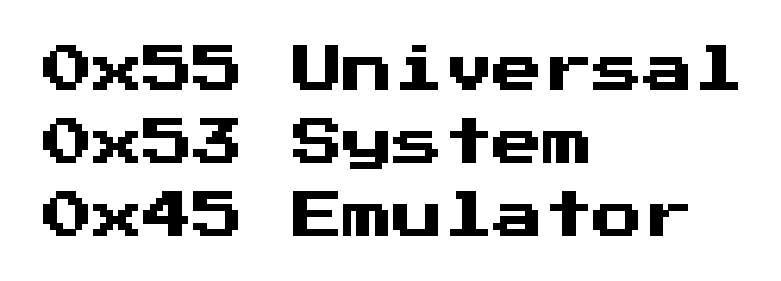
\includegraphics[width=0.5\textwidth]{images/logo-full-path.pdf}
	\end{figure}
	Univerzální emulační platforma
	\begin{itemize}
		\item Jednotný způsob tvorby komponent a~systémů
		\item Libovolná úroveň abstrakce --- cycle-accurate emulace
		\item Připravena snadná tvorba GUI a~zvukového výstupu
		\item Multiplatformní --- GNU/Linux, macOS, Windows\dots
		\item Moderní toolchain: C++20, CMake, CTest, Sphinx
		\item Snadno přístupné: open-source na GitHubu
		\begin{itemize}
			\item Dostupné na~\url{https://golas.me/use/}
			\item Dokumentace na~\url{https://golas.me/usedocs/}
		\end{itemize}
	\end{itemize}
\end{frame}

\begin{frame}
	\frametitle{Webová dokumentace}
	\begin{figure}
		\centering
		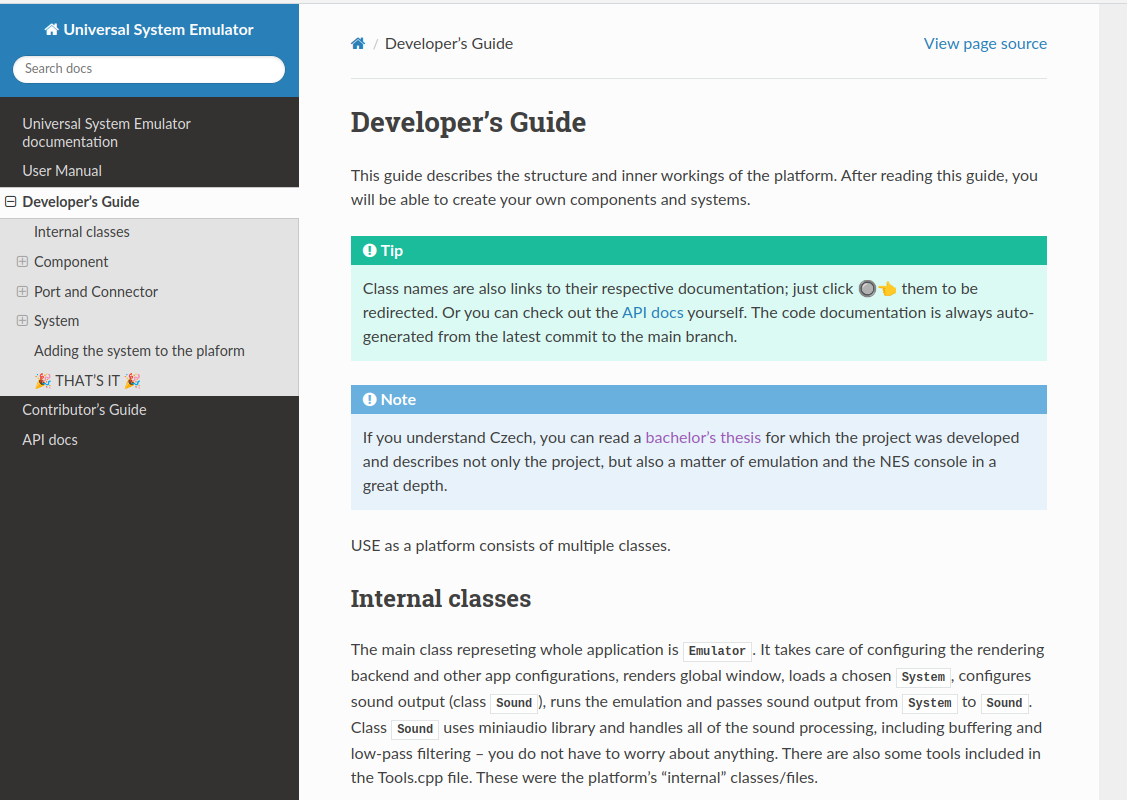
\includegraphics[width=0.8\textwidth]{images/docs.png}
		\caption{\normalsize Webová dokumentace k~projektu}
	\end{figure}
\end{frame}

\begin{frame}
	\frametitle{Vlastnosti řešení}
	\begin{figure}
		\centering
		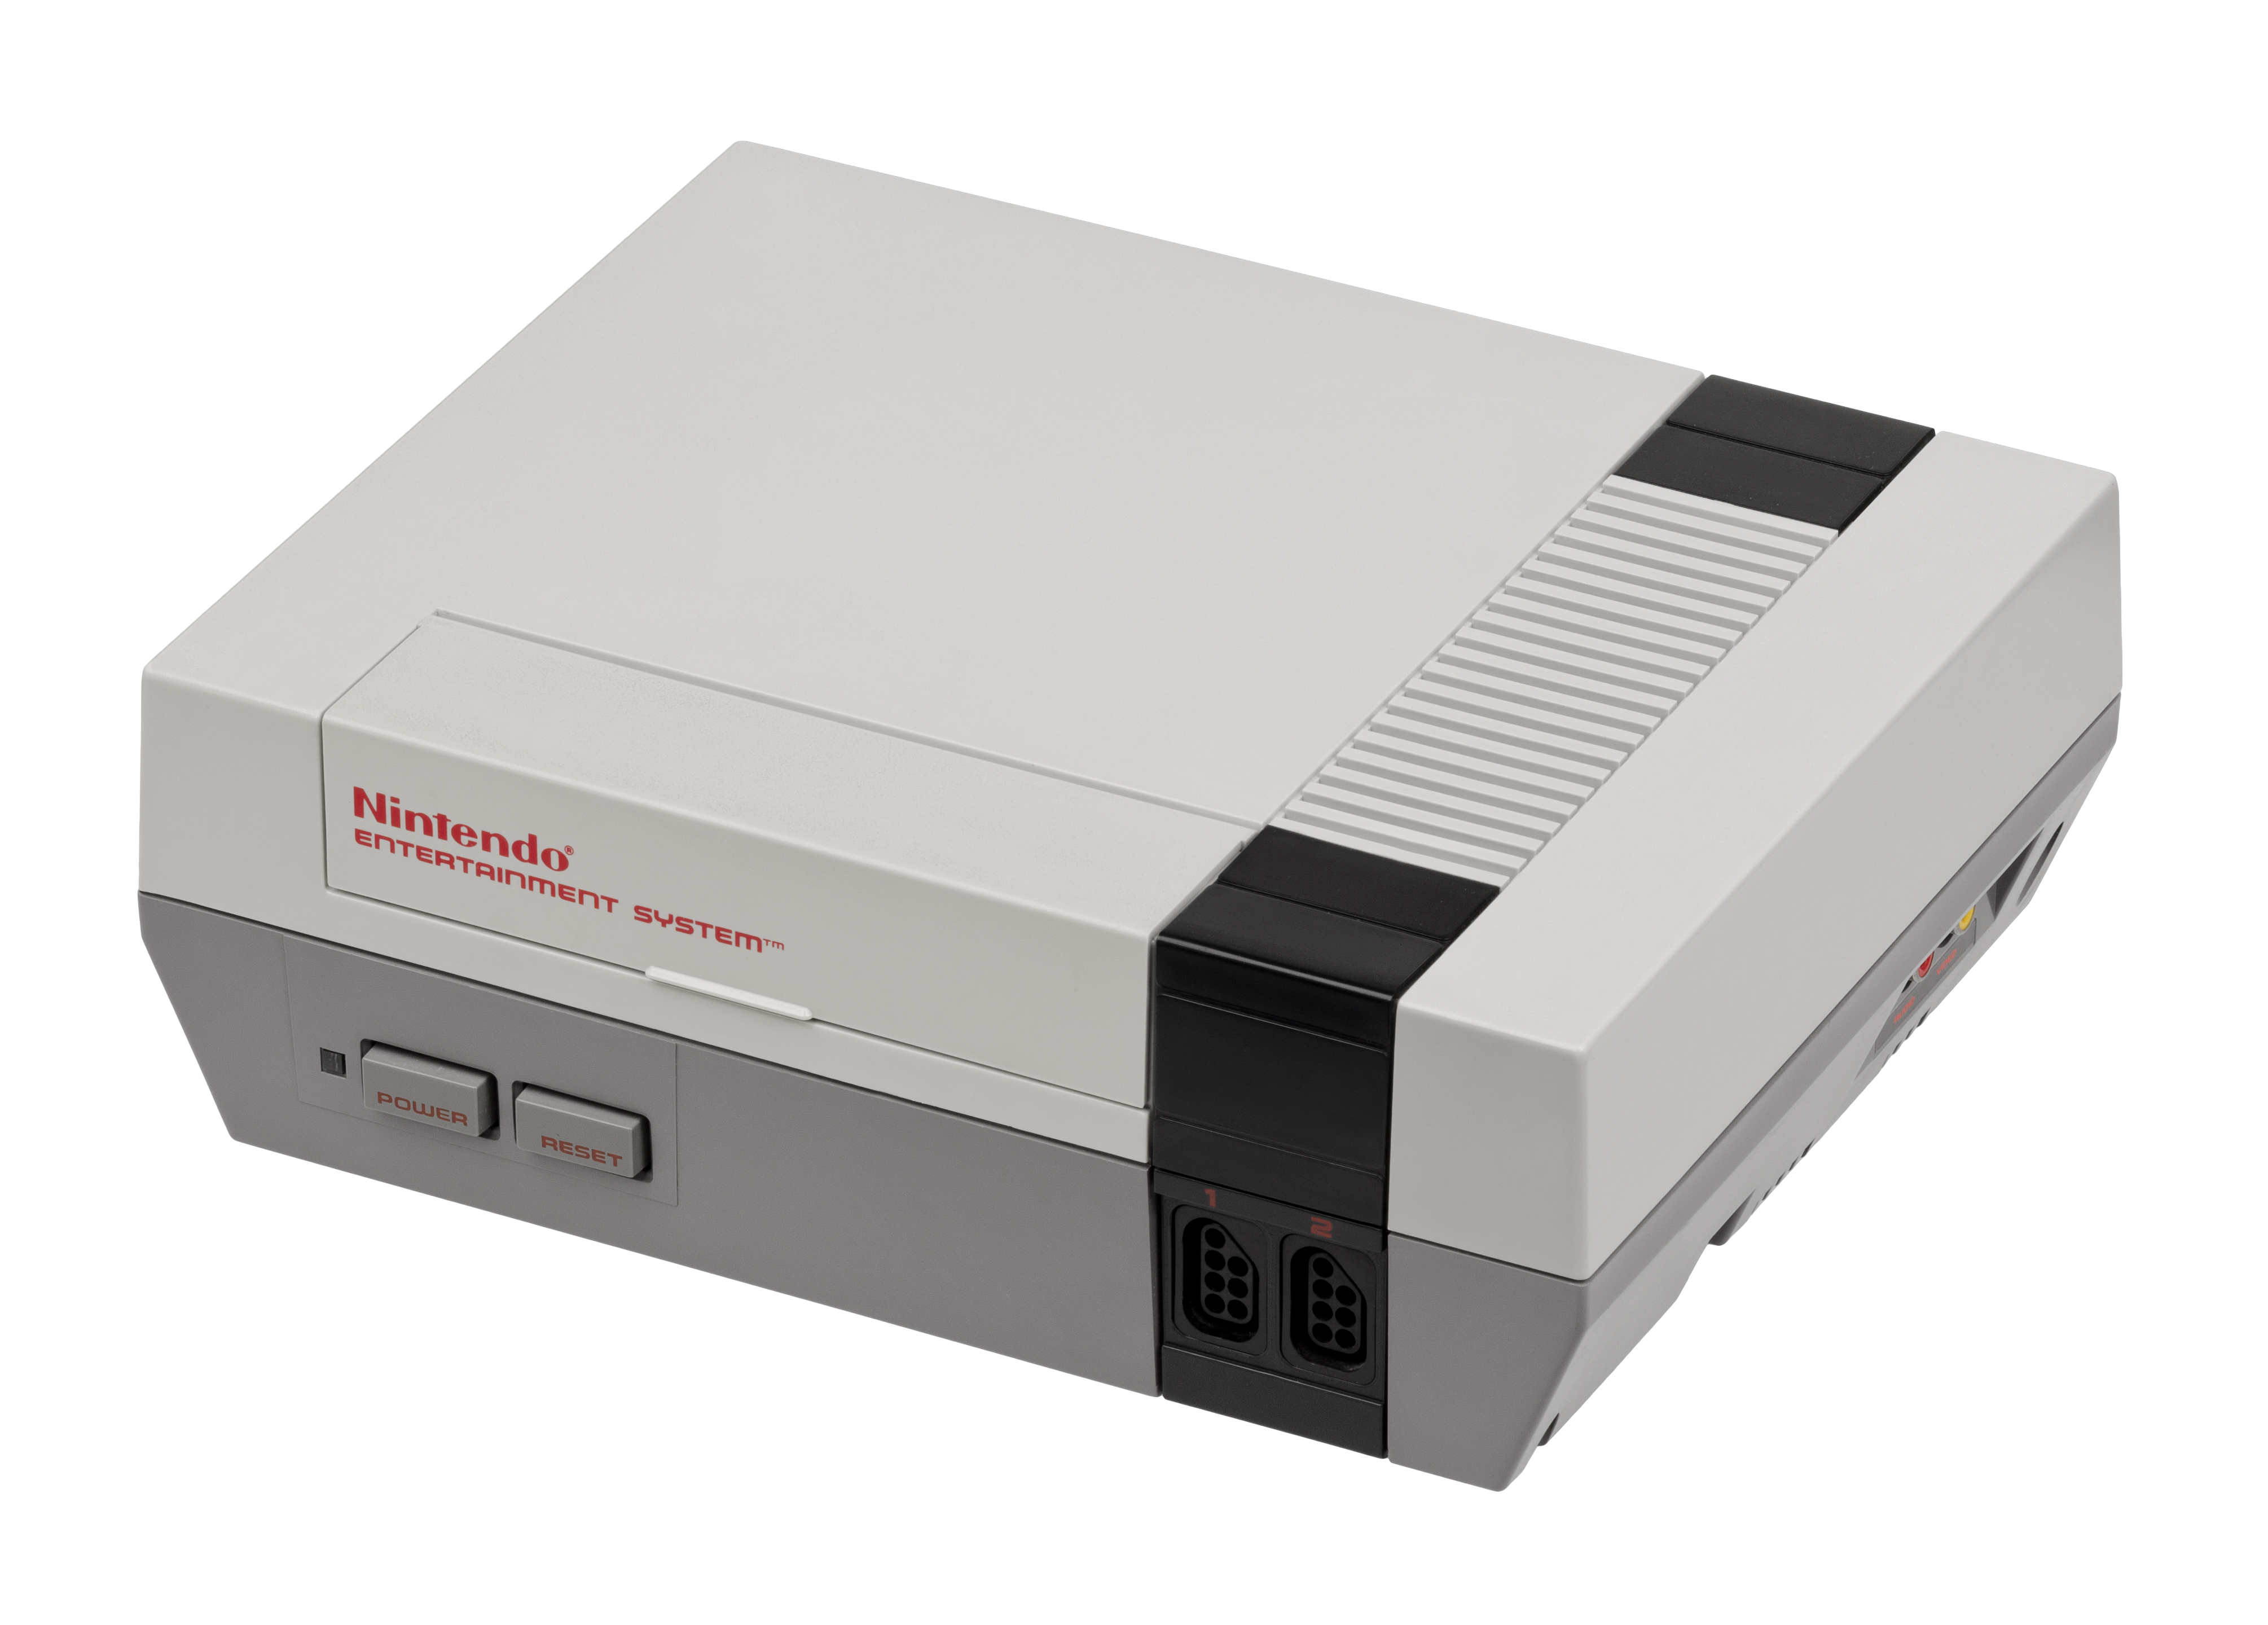
\includegraphics[width=0.25\textwidth]{images/nes.jpg}
		\caption{Konzole NES (foto \copyright~2016, Evan-Amos)}
	\end{figure}
	Emulátor NES:
	\begin{itemize}
		\item Implementovány veškeré komponenty NES
		\item Přehledné zobrazení vnitřních stavů v~emulátoru
		\item Možnost spouštět jednoduché i~složitější hry
		\item Srozumitelný kód, podrobná dokumentace a~manuály
		\item Integrováno do vlastní emulační platformy
	\end{itemize}
\end{frame}

\begin{frame}
	\frametitle{Ukázka}
	\begin{figure}
		\centering
		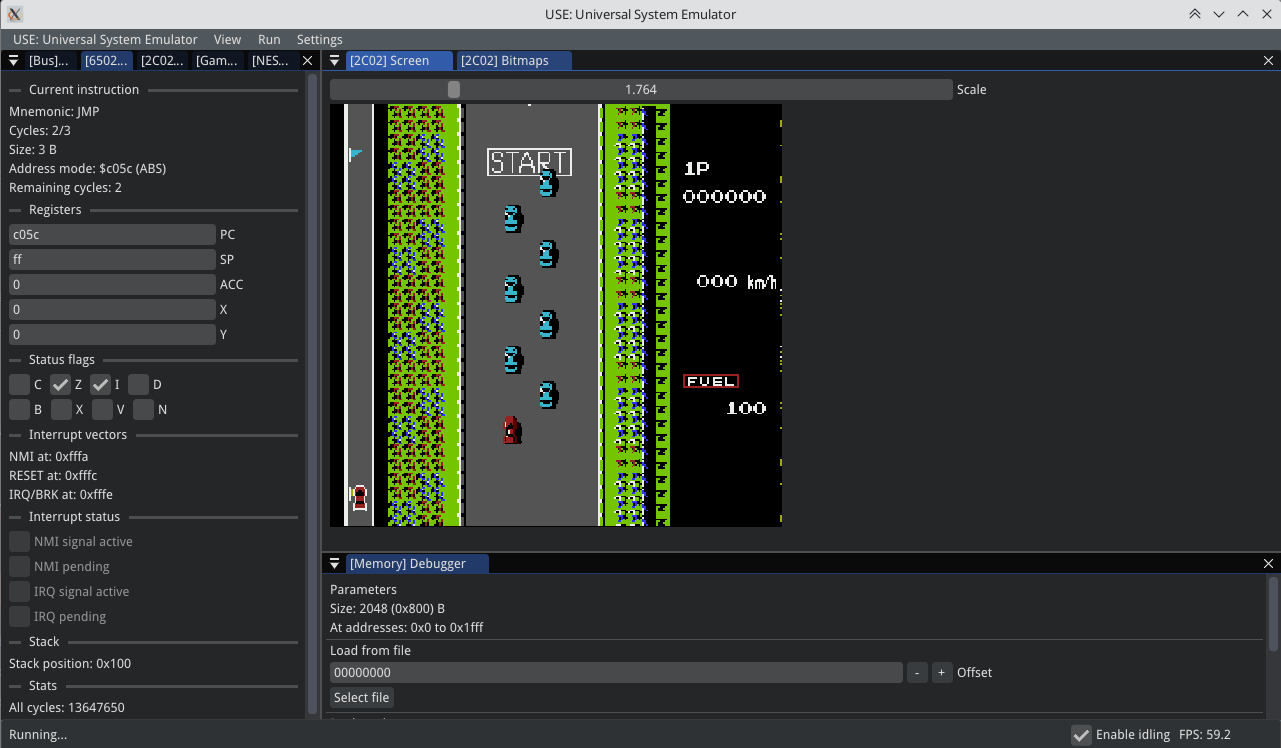
\includegraphics[width=1\textwidth]{images/ss_nes_game_loaded.png}
		\caption{\small Hra \enquote{Road Fighters} spuštěná na emulátoru}
	\end{figure}
\end{frame}

\begin{frame}
	\frametitle{Shrnutí}
	Během 2~let vzniklo následující:
	\begin{itemize}
		\item Přehledný emulátor konzole NES
		\item Podrobná webová dokumentace
		\item Přehled celého procesu vývoje v~textu práce
		\item Nad rámec zadání:
		\begin{itemize}
			\item Platforma pro vývoj emulátorů
			\item Plug-in do grafické knihovny Dear ImGui
			\item Automatické testy pro MOS~6502
		\end{itemize}
	\end{itemize}
	Potenciální navazující práce:
	\begin{itemize}
		\item Využití v~závěrečných pracích (maturitní, bakalářské)
		\item Podpora dalších komponent
		\item Podpora komponent ve Verilogu:
		\begin{itemize}
			\item Emulace RISC-V mikroarchitektur
		\end{itemize}
	\end{itemize}
\end{frame}

\appendix

\begin{frame}
	\frametitle{Otázka oponenta}
	Odhadněte cenu vytvořeného emulátoru.
	\pause
	\begin{itemize}
		\item Byl využit model COCOMO (pokročilý, organický)
		\item Změny v~atributech:
		\begin{table}[ht!]
			\centering
			\begin{tblr}{|Q[c,m]|Q[c,m]|Q[c,m]|Q[c,m]|Q[c,m]|Q[c,m]|}
				\hline
				RELY & DATA & CPLX & TURN & MODP & TOOL \\
				\hline
				H & L & H & L & VH & H \\
				\hline
			\end{tblr}
		\end{table}
		\item Čistý počet řádků kódu: 5~701
		\item Potřebný čas vývoje: 12~měsíců
		\item Průměrná mzda~v IT dle ČSÚ: 73~053~Kč (Q4~2022)
	\end{itemize}
	\pause
	\huge{Celková cena: 2~112~054~Kč}
\end{frame}

\begin{frame}
	\frametitle{Hardware konzole NES}
	\begin{itemize}
		\item Procesor Ricoh 2A03 (klon MOS 6502)
		\item Zvukový syntezátor
		\begin{itemize}
			\item 4 různé kanály
		\end{itemize}
		\item Grafický čip Ricoh 2C02
		\begin{itemize}
			\item Přímo generuje NTSC
			\item Hardware podpora sprajtů
		\end{itemize}
		\item Kazety pro distribuci softwaru
		\begin{itemize}
			\item Obsahují sofistikované mapovací obvody
		\end{itemize}
		\item Periferie (herní ovladače)	
	\end{itemize}
\end{frame}

\begin{frame}
	\frametitle{Diagram tříd platformy}
	\begin{figure}
		\centering
		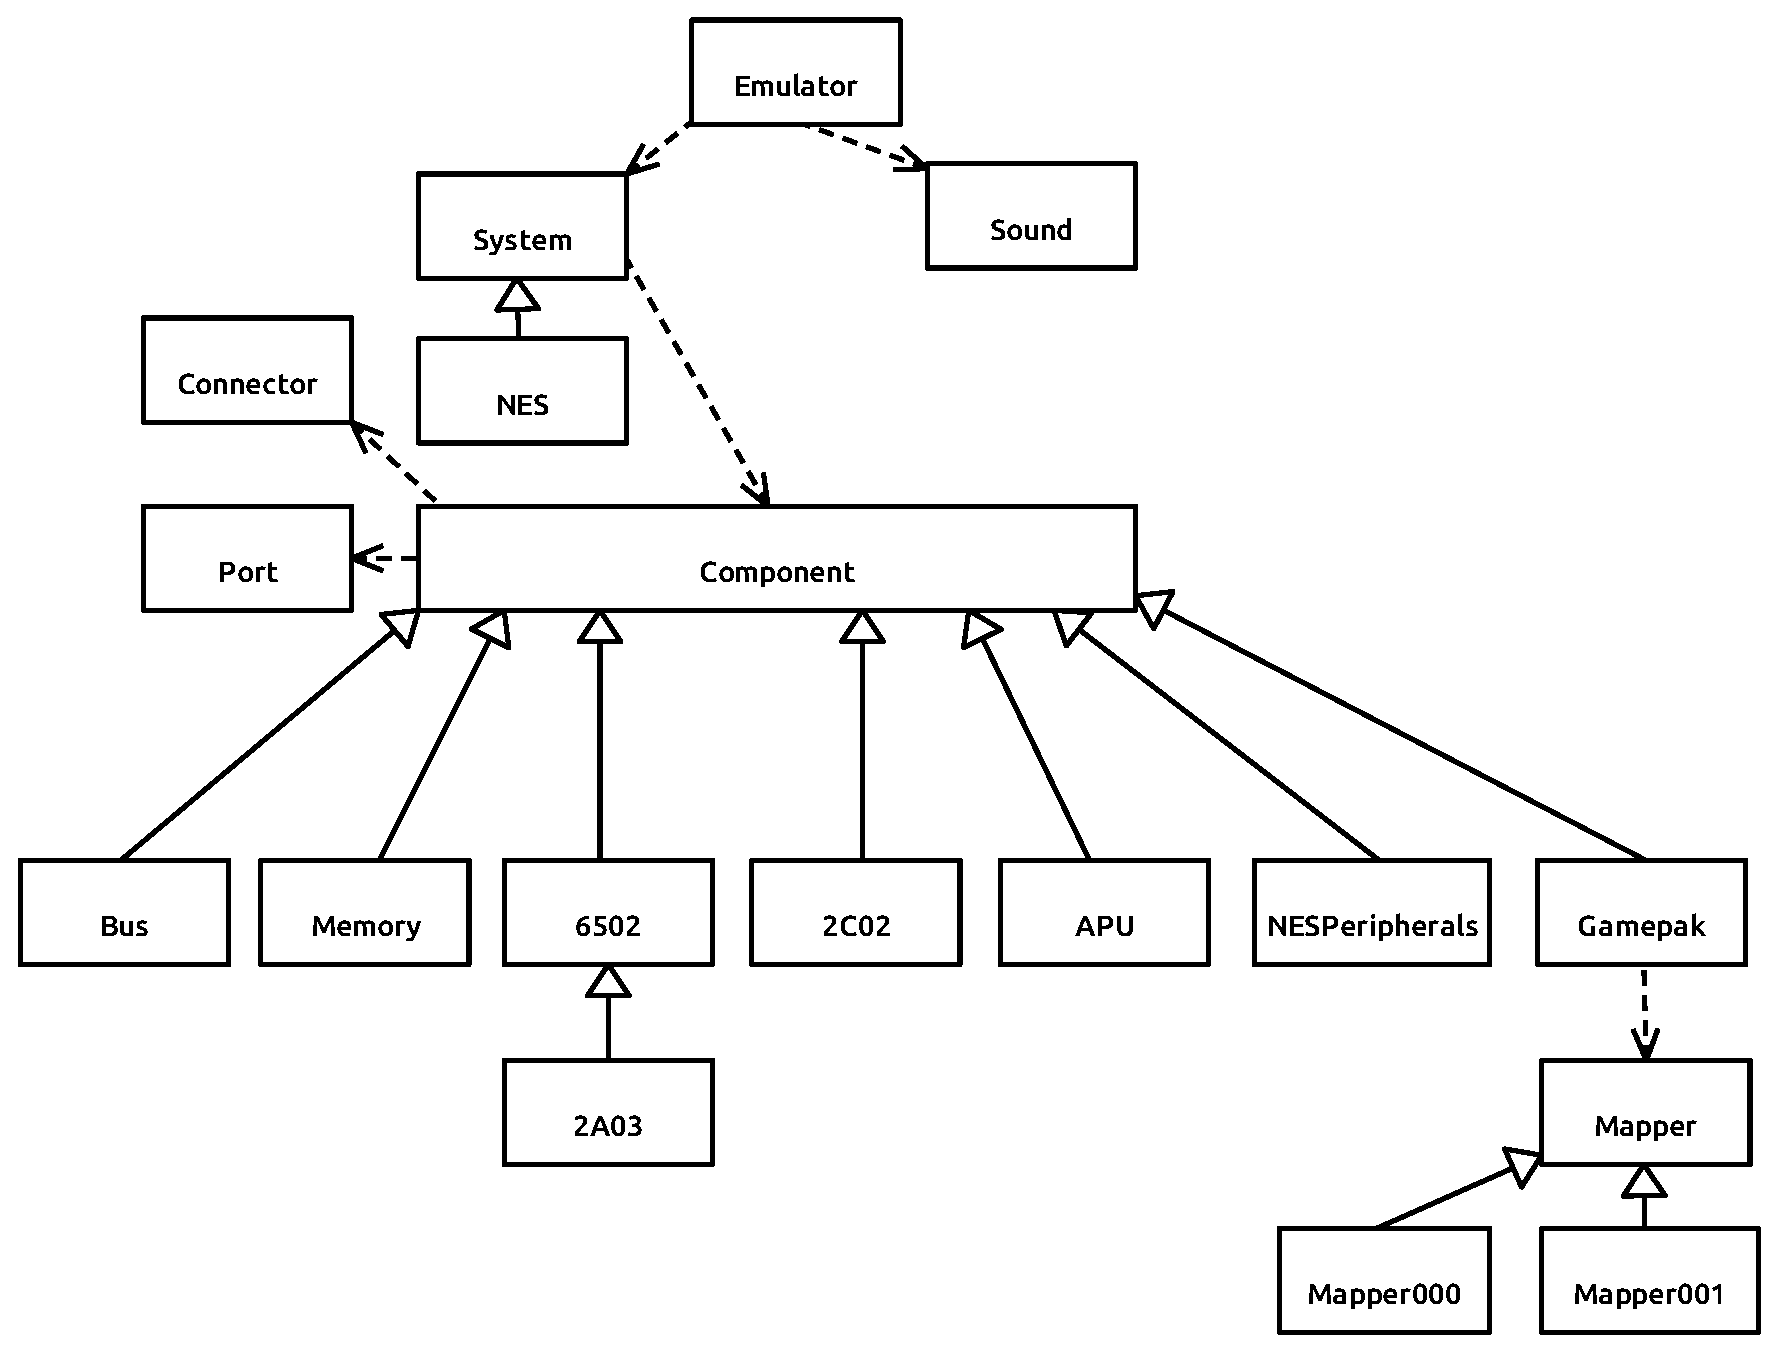
\includegraphics[width=0.8\textwidth]{images/navrh_prehled.pdf}
		\caption{\normalsize Přehledový diagram tříd}
	\end{figure}
\end{frame}
	
\end{document}